%! Author = albert
%! Date = 11.04.2021

% Preamble
\documentclass[11pt]{article}

% Packages
\usepackage[T1]{fontenc}
\usepackage[utf8]{inputenc}
\usepackage{latexsym,amsmath,amssymb,amsthm}
\usepackage{multicol}
\usepackage{graphicx}
\usepackage{geometry}
\usepackage{lipsum}
\usepackage{breqn}
\usepackage{longtable}
\usepackage{enumerate}
\usepackage{subfig}
\usepackage{subfigure}
\usepackage{linegoal}
\usepackage{graphics}
\usepackage{tabularx}
\usepackage{pdflscape}
\usepackage{bm}
\usepackage{empheq}
\usepackage{url}
\usepackage{adjustbox} %dopasowanie tabeli
\usepackage{float} % zmuszanie obrazków do bycia w konkretnym miejscu
\usepackage{floatrow} % kilka obrazków w lini dla float




\renewcommand{\arraystretch}{1,25}

\title{Big Data Analytics\\ Introduction to Complex System\\ Site percolation on the square lattice}
\author{Albert Piekielny 244951\\}
\date{11.04.2021}


%% Uncomment to change margins size
\geometry{top=2.5cm,bottom=2cm,left=2.5cm,right=2.5cm}

\DeclareMathOperator{\sgn}{sgn}
\newcommand{\mA}{\bm{A}}
\newcommand{\mB}{\bm{B}}
\newcommand{\mC}{\bm{C}}
\newcommand{\mL}{\bm{L}}
\newcommand{\mU}{\bm{U}}
\newcommand{\mZ}{\bm{0}}
\newcommand{\vb}{\bm{b}}
\newcommand{\vx}{\bm{x}}
\newcommand{\R}{\mathbb{R}}


% Document
\begin{document}
    \maketitle


    \section{Introduction}
    \label{sec:introduction}

    The site percolation model simulation was written in Java in version 15 with usage of IntelliJ IDE (2021.1).
    All plots ware generated by using python in version 3.8 and with usage of Pycharm IDE (2021.1).
    Computer used for all calculations has the following parameters:
    \begin{itemize}
        \item Intel® Core™ i5-7200U CPU @ 2.50GHz × 4
        \item 16GB RAM memory
        \item 512GB of SSD storage
        \item Ubuntu 20.04.2 LTS 64 bit
    \end{itemize}
    With given parameters: $L=x,\ T=100,\ p0=0.0,\ pk=1.0,\ dp=0.001$ time needed to get result file is:
    \begin{itemize}
        \item $1,55$s for $x = 10$
        \item $23,4$s for $x = 50$
        \item $90,3$s for $x = 100$
    \end{itemize}

    All simulations presented in this document were generated for $T=10^4$ and $d_p = 0.001$


    \section{Presentation results}
    \label{sec:results}

    \subsection{Part I}
    \label{subsec:part-1}

    Visualize sample configurations for $L = 10$ and $3$ values of $p = 0.4,\ 0.6,\ 0.8$ within two methods:
    \begin{itemize}
        \item[(1)] use the burning algorithm and describe each site by the number
        \item[(2)] use the HK algorithm and color each cluster with the different color.
    \end{itemize}


    \begin{figure}[H]
        \centering
        \subfigure[]{
            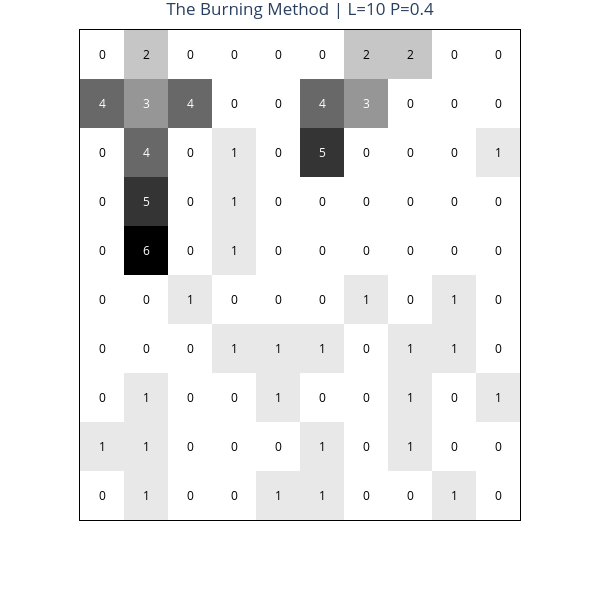
\includegraphics[width=0.47\linewidth]{albi_burning_method_p40}
        }
        \subfigure[]{
            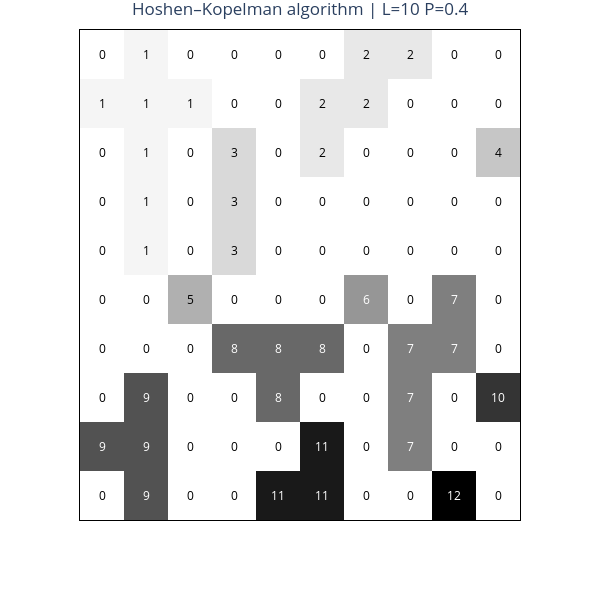
\includegraphics[width=0.47\linewidth]{hk_p40}
        }
        \caption{An example of the burning method (a) and HK algorithm (b) for $p = 0.4$}
        \label{fig:first}
    \end{figure}

    \begin{figure}[H]
        \centering
        \subfigure[]{
            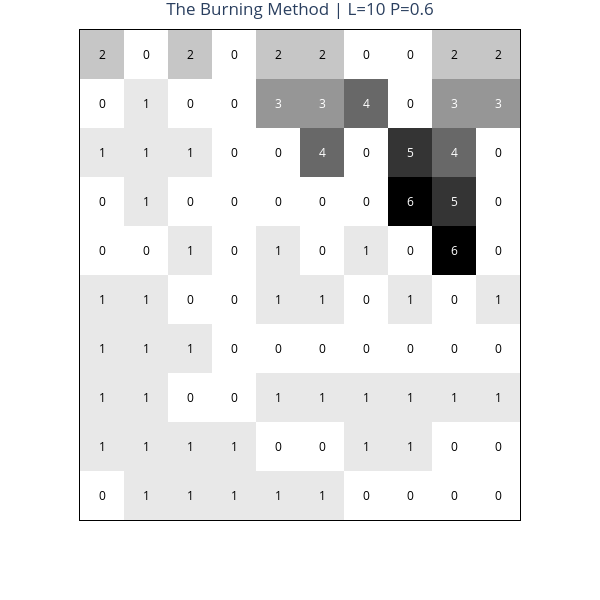
\includegraphics[width=0.47\linewidth]{albi_burning_method_p60}
        }
        \subfigure[]{
            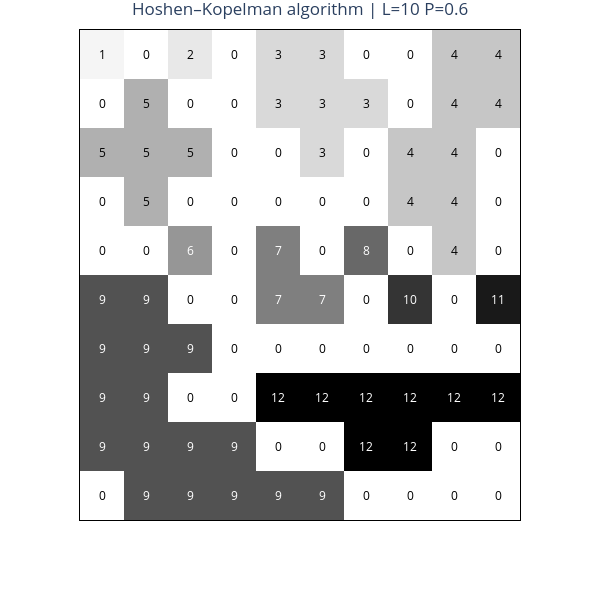
\includegraphics[width=0.47\linewidth]{hk_p60}
        }
        \caption{An example of the burning method (a) and HK algorithm (b) for $p = 0.6$}
        \label{fig:second}
    \end{figure}

    \begin{figure}[H]
        \centering
        \subfigure[]{
            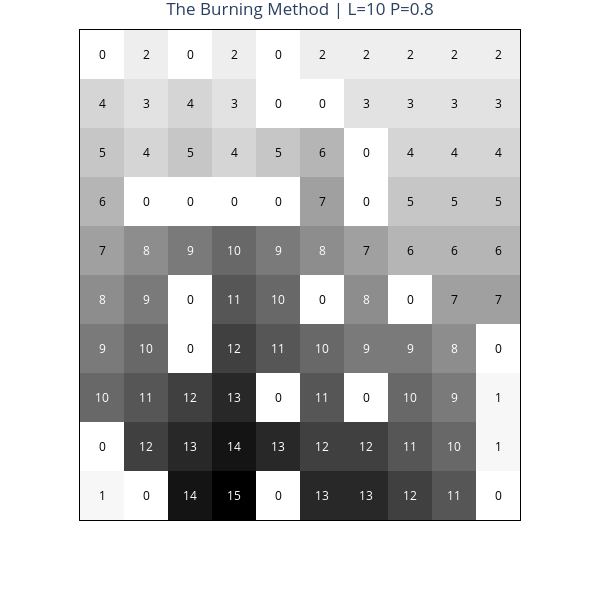
\includegraphics[width=0.47\linewidth]{albi_burning_method_p80}
        }
        \subfigure[]{
            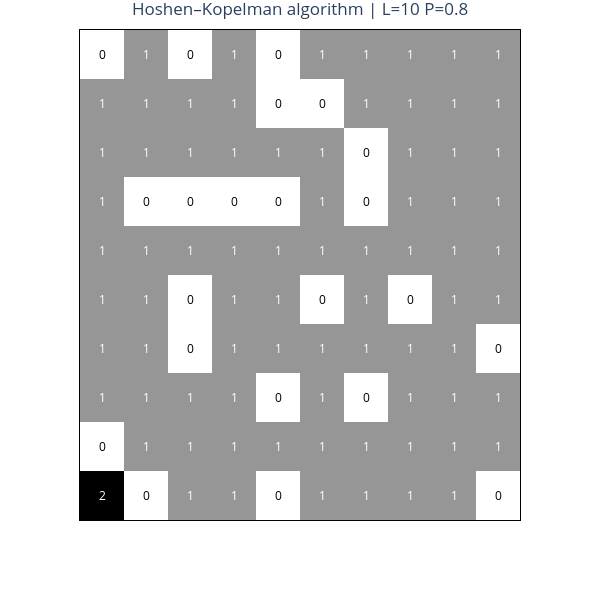
\includegraphics[width=0.47\linewidth]{hk_p80}
        }
        \caption{An example of the burning method (a) and HK algorithm (b) for $p = 0.8$}
        \label{fig:third}
    \end{figure}

    \subsection{Part II}
    \label{subsec:part-b}
    Present $P_flow$ (that the path connecting the first and the last row exists) as a function of
    p for $L = 10,\ 50,\ 100$ and for $T = 10^4$ .

    \begin{figure}[H]
        \centering
        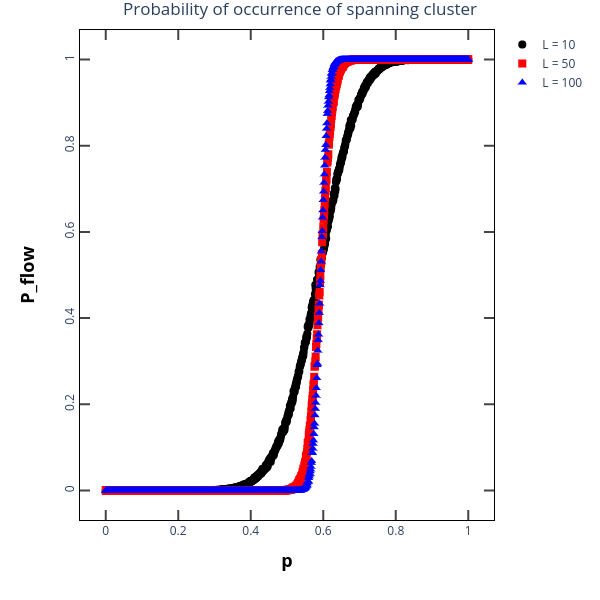
\includegraphics[width=0.60\linewidth]{Pflow}
        \caption{Probability P f low that the path connecting the first and the last row
        exists as a function of p for $L = 10,\ 50,\ 100$}
        \label{fig:fourth}
    \end{figure}

    \subsection{Part III}
    \label{subsec:part-c}
    Present average size of the maximum cluster as a function of p for L = 10, 50, 100 and for $T = 10^4$.
    \begin{figure}[H]
        \centering
        \subfigure[]{
            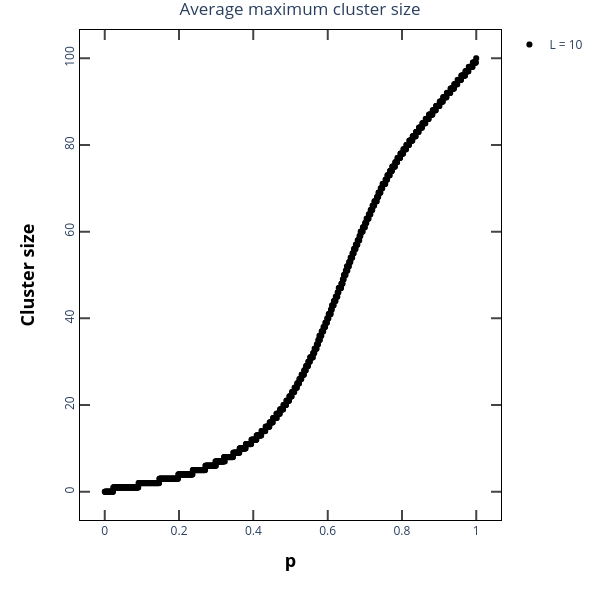
\includegraphics[width=0.47\linewidth]{avg_cluster_size_10}
        }
        \subfigure[]{
            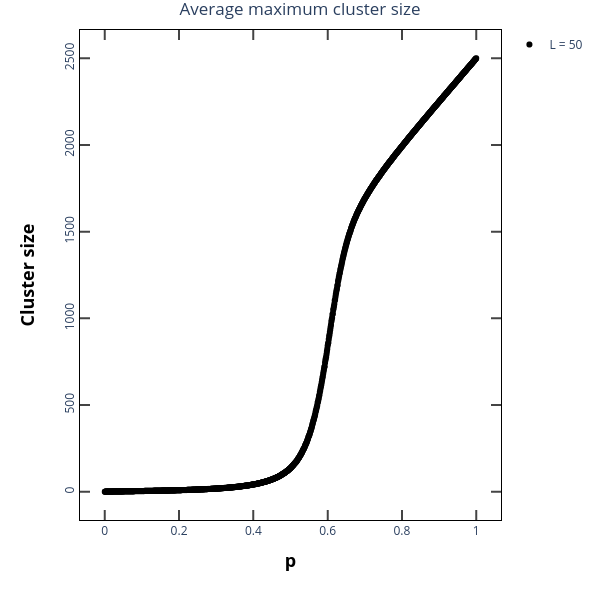
\includegraphics[width=0.47\linewidth]{avg_cluster_size_50}
        }
        \bigskip
        \subfigure[]{
            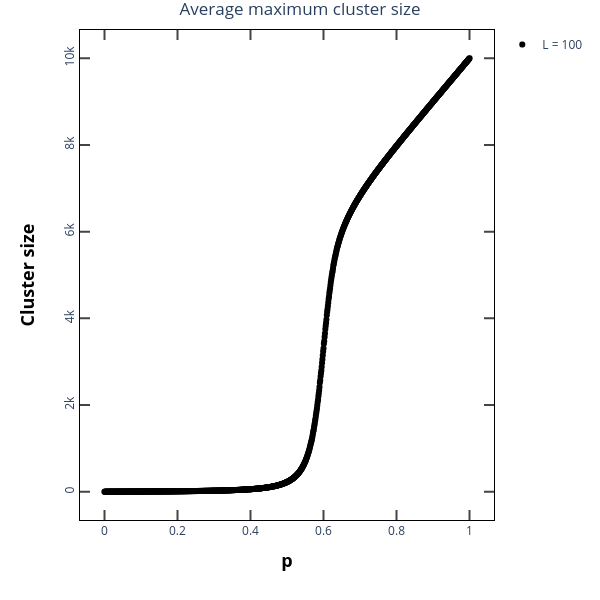
\includegraphics[width=0.47\linewidth]{avg_cluster_size_100}
        }
        \subfigure[]{
            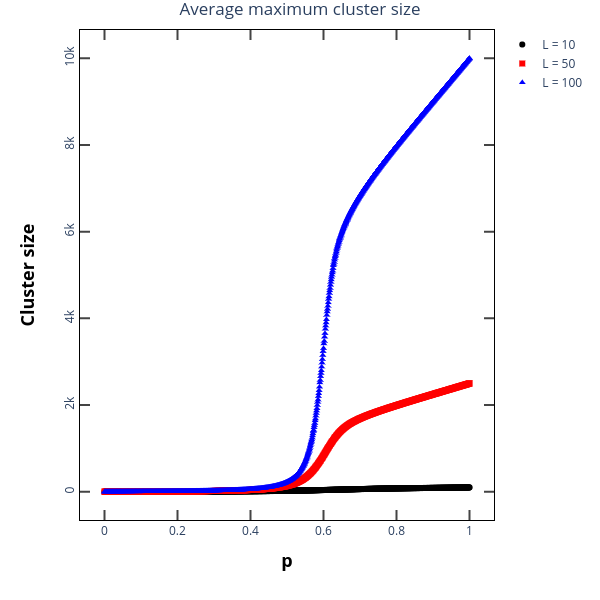
\includegraphics[width=0.47\linewidth]{avg_cluster_size_all}
        }
        \caption{Graphs a, b, c show the average size of the maximum cluster size for $L = 10,\ L = 50,\ L = 100$
            respectively. Graph d shows the overlapping graphs.}
        \label{fig:fifth}
    \end{figure}

    \subsection{Part IV}
    \label{subsec:part-d}
    Present distribution of clusters $n(s, p, L)$ for a given $p : 0.2,\ 0.3,\ 0.4,\ 0.5,\ 0.592746,\ 0.6,\ 0.7,\ 0.8.$

    \begin{figure}[H]
        \centering
        \subfigure[]{
            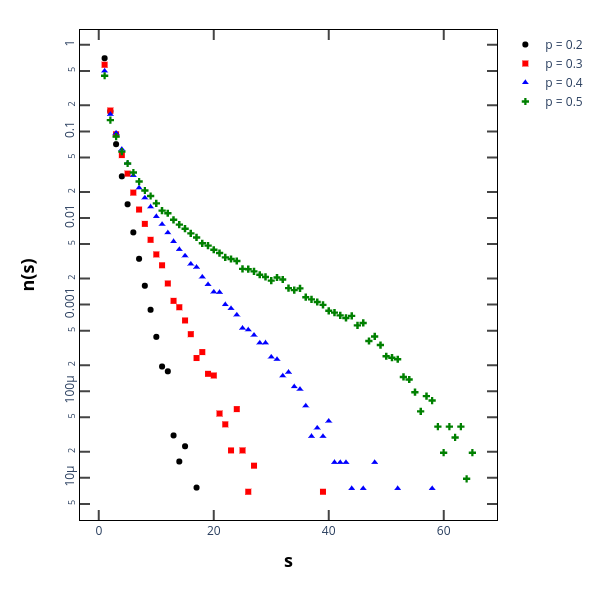
\includegraphics[width=0.47\linewidth]{distribuantion_l10_1}
        }
        \bigskip
        \subfigure[]{
            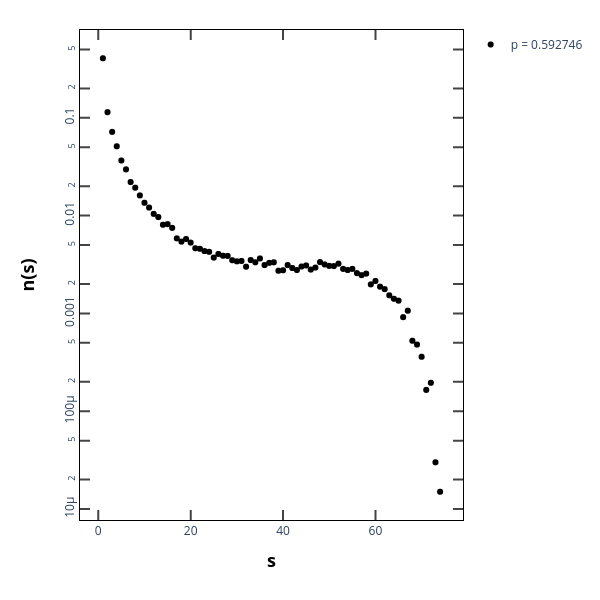
\includegraphics[width=0.47\linewidth]{distribuantion_l10_2}
        }
        \bigskip
        \subfigure[]{
            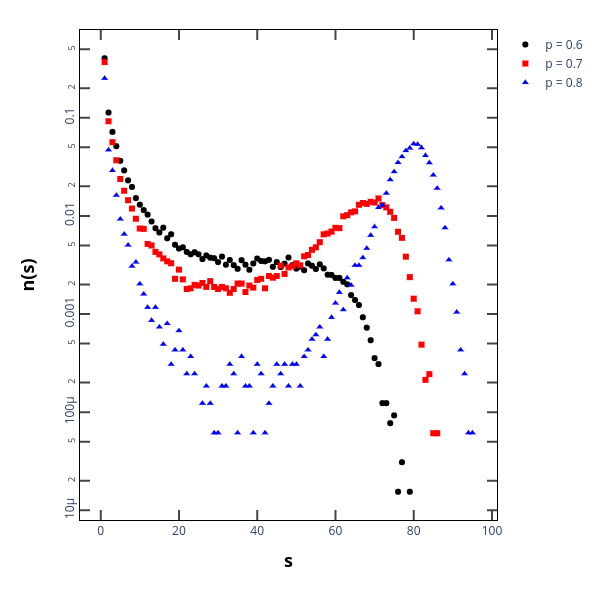
\includegraphics[width=0.47\linewidth]{distribuantion_l10_3}
        }

        \caption{Cluster size distributions for square lattice, for $p < p_c$ (a), $p = p c = 0.592746$ (b)
            and $p > p_c$ (c), with $L = 10$, averaged over $T = 10^4$ trials.}
        \label{fig:sixth}
    \end{figure}

    \newpage
    \begin{figure}[H]
        \centering
        \subfigure[]{
            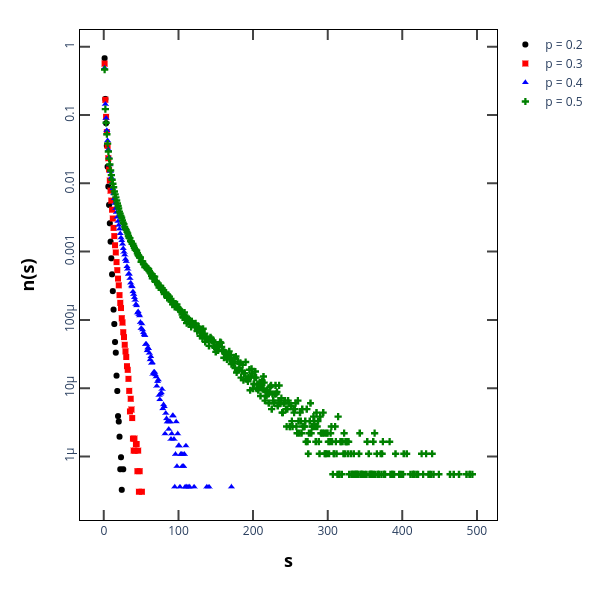
\includegraphics[width=0.47\linewidth]{distribuantion_l50_1}
        }
        \bigskip
        \subfigure[]{
            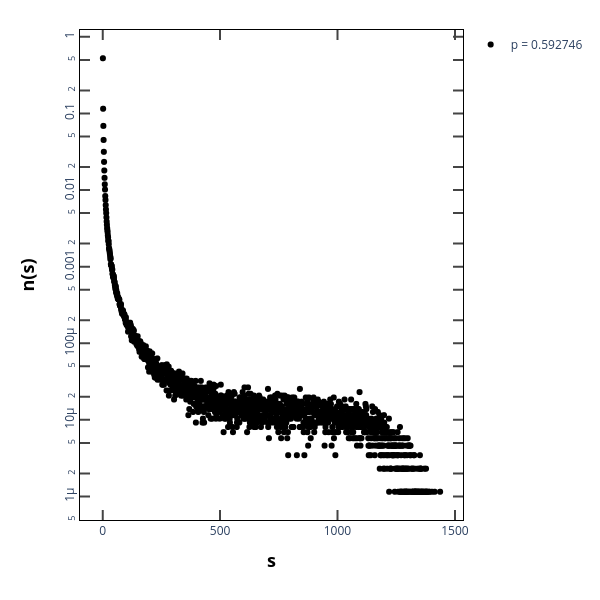
\includegraphics[width=0.47\linewidth]{distribuantion_l50_2}
        }
        \bigskip
        \subfigure[]{
            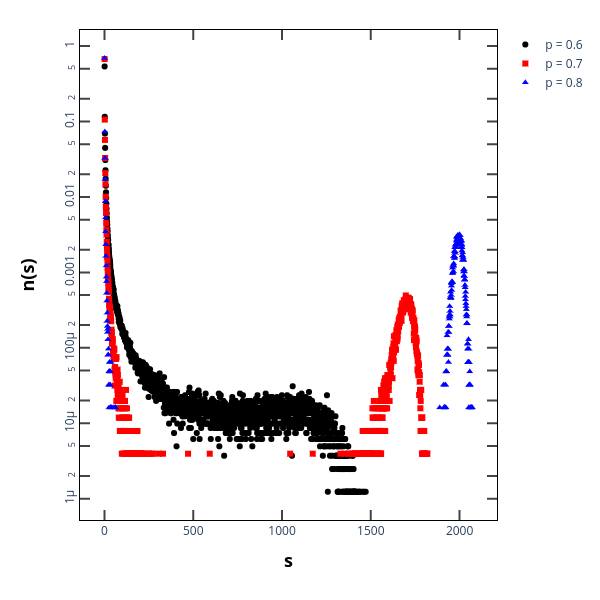
\includegraphics[width=0.47\linewidth]{distribuantion_l50_3}
        }

        \caption{Cluster size distributions for square lattice, for $p < p_c$ (a), $p = p c = 0.592746$ (b)
            and $p > p_c$ (c), with $L = 50$, averaged over $T = 10^4$ trials.}
        \label{fig:seventh}
    \end{figure}

    \newpage
    \begin{figure}[H]
        \centering
        \subfigure[]{
            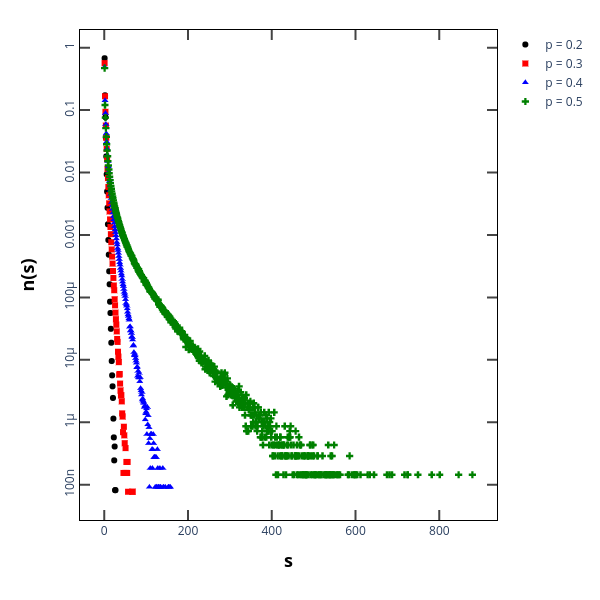
\includegraphics[width=0.47\linewidth]{distribuantion_l100_1}
        }
        \bigskip
        \subfigure[]{
            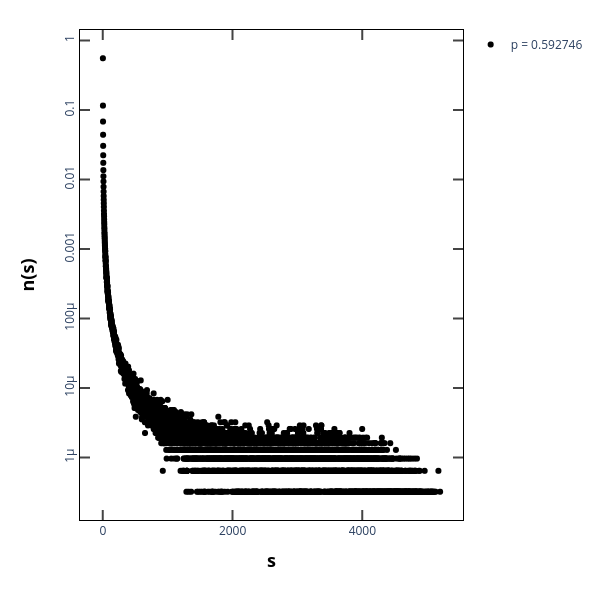
\includegraphics[width=0.47\linewidth]{distribuantion_l100_2}
        }
        \bigskip
        \subfigure[]{
            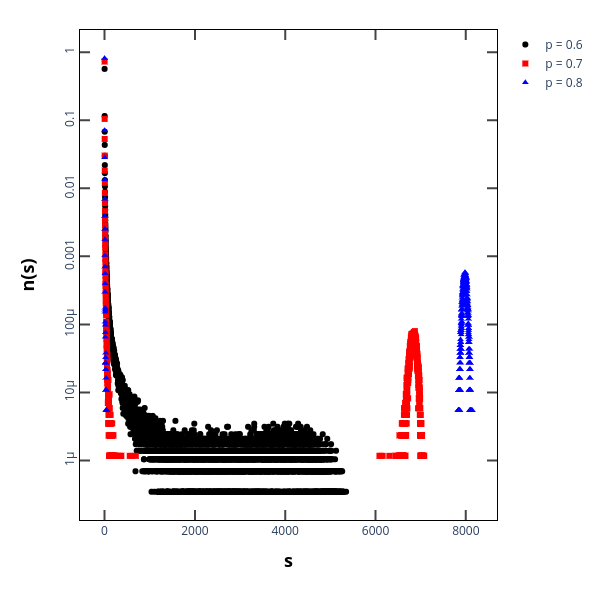
\includegraphics[width=0.47\linewidth]{distribuantion_l100_3}
        }

        \caption{Cluster size distributions for square lattice, for $p < p_c$ (a), $p = p c = 0.592746$ (b)
            and $p > p_c$ (c), with $L = 100$, averaged over $T = 10^4$ trials.}
        \label{fig:eigth}
    \end{figure}


\end{document}